% Ejercicio 1
\begin{ejer}
Sea $\dot{x} = f(x) g(t)$ una ecuación de variables separables; demostrar que,
si la ecuación no es $\dot{x} = 0$ (en cuyo caso todos los puntos son de
equilibrio) entonces los puntos de equilibrio son exactamente los ceros
de $f$. Hallar los puntos de equilibrio y resolver las siguientes ecuaciones
diferenciales de variables separables:
\[
    (\text{a})\quad \dot{x} = x^2 - 1, \qquad
    (\text{b})\quad \dot{x} = \frac{1}{t^2 - 1}, \qquad
    (\text{c})\quad \dot{x} = x^2 \cos t, \qquad
    (\text{d})\quad \dot{x} = a(t)x.
\]
\end{ejer}
\begin{sol}
Es inmediato que si $x_0$ es cero de $f$, entonces $f(x_0)g(t) = 0$ para todo $t \en \mathbb{R}$, por lo que $x_0$ es punto de equilibrio. Recíprocamente, si $x_0$ es punto de equilibrio, entonces $f(x_0)g(t) = 0$ para todo $t \en \mathbb{R}$, pero la ecuación no es $\dot{x} = 0$, por lo cual tiene que existir un $t_0 \en \mathbb{R}$ tal que $g(t_0) \neq 0$; luego, se tiene que $f(x_0)g(t_0) = 0$ con $g(t_0) \neq 0$, de esto se sigue que $f(x_0) = 0$. Esto concluye la prueba. Ahora encontremos los puntos de equilibrio y las soluciones de cada EDO:
\begin{enumerate}[label = (\alph*)]
    \item Por lo visto al inicio, los puntos de equilibrio son los ceros de $x^2 -1$, i.e., $\set{1,-1}$; por lo tanto, por los puntos de la forma $(t_0, 1)$ y $(t_0, -1)$ pasan, respectivamente, las soluciones constantes $\varphi(t) = 1$ y $\varphi(t) = -1$ definidas sobre todo $\mathbb{R}$. Ahora encontremos una solución que pasa por un punto arbitrario $(t_0, x_0) \en \mathbb{R}^2$ con $x_0 \notin \set{1,-1}$: si $\varphi(t)$ es solución y $\varphi(t_0) = x_0$, entonces ---gracias a que $x^2 - 1$ es localmente Lipschitz--- $\varphi(t)$ no cruza las rectas $x = \pm 1$. Luego,
    \[
        \frac{\dot{\varphi}(t)}{\varphi(t)^2 - 1} = 1%
        \implies%
        \int^t_{t_0} \frac{\dot\varphi(s) \mathrm{d}s}{\varphi(s)^2 - 1} = t - t_0
    \]
    usando cambio de variable y el hecho de que $\frac{1}{x^2 - 1} = \frac12\left(\frac{1}{x-1} - \frac{1}{x+1}\right)$, llegamos a que 
    \begin{align*}
        t - t_0%
        &= \int^{\varphi\mathrlap{(t)}}_{{x_0}} \frac{\mathrm{d}x}{x^2 - 1}%
        = \frac12 \left(%
            \int^{\varphi\mathrlap{(t)}}_{{x_0}} \frac{\mathrm{d}x}{x - 1} - \int^{\varphi\mathrlap{(t)}}_{{x_0}} \frac{\mathrm{d}x}{x + 1}
        \right)\\
        &= \frac12 \big(%
            \ln|\varphi(t) - 1| - \ln|x_0 - 1| - \ln|\varphi(t) + 1| + \ln|x_0 + 1|
        \big)\\
        &= \frac12\ln\left|%
            \frac{(\varphi(t) - 1)(x_0 + 1)}{(\varphi(t) + 1)(x_0 - 1)}
        \right|
    \end{align*}
    Despejando $\varphi(t)$ concluimos que la solución es
    \[
        \varphi(t) = \frac{%
            1 + \big(\frac{x_0-1}{x_0+1}\big) e^{2(t-t_0)}
        }{%
            1 - \big(\frac{x_0-1}{x_0+1}\big) e^{2(t-t_0)}
        }
    \]
    Más aún, cuando $|x_0| < 1$ el denominador jamás se anula, por lo que $\varphi(t)$ está definida en todo $\mathbb{R}$. Por otro lado, cuando $|x_0| > 1$ el denominador se anulará en $T = t_0 + \frac12 \ln\big(\frac{x_0 + 1}{x_0 - 1}\big)$ y, en el caso $x_0 > 1$, $\varphi(t)$ estará definida en $]{-\infty}, T[$; mientras que en el caso $x_0 < -1$, $\varphi(t)$ estará definida en $]T, +\infty[$.

    \item Esta EDO no tiene puntos de equilibrio. Dado un punto arbitrario $(t_0, x_0) \en (\mathbb{R}\setminus\set{1,-1}) \times \mathbb{R}$ y una solución $\varphi(t)$ que pasa por dicho punto (definida en un intervalo), se tiene que
    \[
        \dot\varphi(t) = \frac{1}{t^2-1}%
        \implies%
        \int^{t}_{t_0} \dot\varphi(s) \mathrm{d}s = \int^{t}_{t_0} \frac{\mathrm{d}s}{s^2 - 1}
    \]
    lo cual, como ya vimos en el inciso (a), se convierte en 
    \[
        \varphi(t) - x_0%
        = \frac12\ln\left|%
            \frac{t - 1}{t + 1}
        \right| - \frac12\ln\left|%
            \frac{t_0 - 1}{t_0 + 1}
        \right|
    \]
    por lo tanto, la solución es de la forma 
    \[
        \varphi(t)%
        = \frac12\ln\left|%
            \frac{t - 1}{t + 1}
        \right| - \frac12\ln\left|%
            \frac{t_0 - 1}{t_0 + 1}
        \right| + x_0
    \]
    Esta solución está definida en la componente conexa de $\mathbb{R}^2\setminus\set{1,-1}$ a la que pertenece $t_0$.

    \item Por lo visto al inicio, el único punto de equilibrio es el origen; luego, por los puntos de la forma 
    $(t_0,0)$ pasa la solución constante $\varphi(t) = 0$ definida sobre todo 
    $\mathbb{R}$. Ahora encontremos una solución que pasa por un punto arbitrario 
    $(t_0,x_0) \en \mathbb{R}^2$ con $x_0 \neq 0$: si $\varphi(t)$ es solución y 
    $\varphi(t_0) = x_0$, entonces ---gracias a que $x^2 \cos(t)$ es localmente 
    Lipschitz en $x$--- la solución $\varphi(t)$ no cruza la recta $x=0$. Luego,
    \[
        \frac{\dot{\varphi}(t)}{\varphi(t)^2}%
        = \cos(t)%
        \implies%
        \int^t_{t_0} \frac{\dot\varphi(s)}{\varphi(s)^2}\,\mathrm{d}s 
        = \int^t_{t_0} \cos(s)\,\mathrm{d}s%
        = \sin(t) - \sin(t_0)
    \]
    Usando el cambio de variable se obtiene
    \[
        \sin(t) - \sin(t_0)%
        = \int^{\varphi(t)}_{x_0} \frac{\mathrm{d}x}{x^2}%
        = -\frac{1}{\varphi(t)} + \frac{1}{x_0}
    \]
    Despejando $\varphi(t)$ concluimos que la solución es
    \[
        \varphi(t) = \frac{1}{x_0^{-1} + \sin(t_0) - \sin(t)}
    \]
    Notemos que el denominador se anula en los puntos $A_{t_0,x_0} = \set*{\sin^{-1}\!\big(x_0^{-1} + \sin t_0\big) + 2k\pi \given k \en \mathbb{Z}}$ por lo que el dominio de $
    \varphi$ será el sub-intervalo de $\mathbb{R} \setminus A_{t_0,x_0}$ al que pertenezca $t_0$.

    \item Si $a(t) \equiv 0$, las soluciones son las funciones constantes. Si suponemos entonces que $a$ no es idénticamente cero, el único punto de equilibrio es el origen y, por tanto, por los puntos de la forma $(t_0, 0)$ pasa la solución $\varphi(t) \equiv 0$ definida en $\mathbb{R}$. Como $a(t)x$ es localmente Lipschitz en $x$, cualquier sol. $\varphi$ que pase por un punto $(t_0, x_0)$ con $x_0 \neq 0$ no cruzará el eje $x$, luego
    \[
        \frac{\dot\varphi(t)}{\varphi(t)} = a(t)%
        \implies%
        \int^{t}_{t_0}\frac{\dot\varphi(s)}{\varphi(s)}\mathrm{d}s = \int^{t}_{t_0} a(s)\mathrm{d}s
    \]
    Esto se reduce, usando cambio de variable y definiendo $\operatorname{A}_{t_0}(t) \coloneq \int^{t}_{t_0} a(t)\mathrm{d}t$, a la expresión
    \[
        \ln\left|%
            \frac{\varphi(t)}{x_0}
        \right|%
        = \operatorname{A}_{t_0}(t)
    \]
    por lo que $\varphi(t) = x_0 e^{\operatorname{A}_{t_0}(t)}$ es la sol. definida sobre todo $\mathbb{R}$ siempre que $a \en \operatorname{C}^0(\mathbb{R})$ (TFC).\qedhere
\end{enumerate}
\end{sol}




% Ejercicio 2
\begin{ejer}
Hallar todas las soluciones de la ecuación diferencial
$
    \dot{x} = |x|^{1/2}.
$
\end{ejer}
\begin{sol}
El único punto de equilibrio es el origen, por lo que las funciones constantes $\varphi \equiv 0$ son soluciones definidas sobre todo $\mathbb{R}$. Por otro lado, la función $|x|^{1/2}$ es localmente Lipschitz en $\mathbb{R}\setminus\set0$; sin embargo, no lo es en cero,\footnote{Pues la derivada por la derecha de cero diverge a $+\infty$ y por la izquierda a $-\infty$.} por lo cual podemos analizar las soluciones en cada uno de los intervalos $I_- \coloneq {]{-\infty},0[}$ y $I_+ \coloneq {]0, +\infty[}$.
\begin{itemize}
    \item Si $\varphi$ es una sol. dentro de $\mathbb{R} \times I_+$ que pasa por un punto $(t_0,x_0) \en \mathbb{R} \times I_+$, entonces cumple que $\dot\varphi(t) = |\varphi(t)|^{1/2} = \varphi(t)^{1/2}$. Luego,
    \[
        \frac{\dot\varphi(t)}{\varphi(t)^{1/2}} = 1%
        \implies%
        \int^{t}_{t_0} \frac{\dot\varphi(s)}{\varphi(s)^{1/2}}\mathrm{d}s = t - t_0
    \]
    por lo cual, 
    \[
        2\big(%
            \sqrt{\varphi(t)} - \sqrt{x_0}
        \big) = t - t_0
    \]
    lo que despejando se convierte en
    \[
        \varphi(t)%
        = \frac14 \big(%
            t - t_0 + 2\sqrt{x_0}
        \big)^2%
        = \frac14 \big(%
            t - T
        \big)^2%
        \quad\text{donde}\quad%
        T \coloneq t_0 - 2\sqrt{x_0}
    \]
    Aunque esta función está definida sobre todos los reales, solo resuelve la EDO cuando $t > T$, pues la derivada es $\dot\varphi(t) = \frac12 (t-T) = \frac12|t-T| = |\varphi(t)|^{1/2}$ solo si $t > T$. Esto quiere decir que $\varphi$ se puede definir en $]T, +\infty[$.

    \item Análogamente, si $\varphi$ es sol. dentro de $\mathbb{R} \times I_-$ y pasa por un punto $(t_1,x_1) \en \mathbb{R} \times I_-$, entonces $\dot\varphi(t) = (-\varphi(t))^{1/2}$. Luego, se llega a que 
    \[
        -2\Big(%
            \sqrt{-\varphi(t)} - \sqrt{-x_1}
        \Big)%
        = t - t_1
    \]
    Lo cual al despejar se convierte en 
    \[
        \varphi(t)%
        = -\frac14 \big(%
            t - t_1 - 2\sqrt{-x_1}
        \big)^2%
        = -\frac14 \big(%
            t-T'
        \big)^2%
        \quad\text{donde}\quad%
        T' \coloneq t_1 + 2\sqrt{-x_1}
    \]
    De forma similar al punto anterior, $\varphi$ se puede definir sobre $]{-\infty},T'[$.
\end{itemize}
De este modo, las soluciones maximales de la ecuación original se construyen pegando las tres soluciones encontradas. Es decir, son de la forma
\[
\varphi(t) =%
\begin{cases}
    -\frac14\big(t - T'\big), & \text{si } t \leq T',\\
    0,  & \text{si } T' \leq t \leq T\\
    \frac14\big(t - T\big), & \text{si } t \geq T
\end{cases}
\]
Ya vimos que $\varphi$ es sol. en el interior de cada uno de los $3$ sub-intervalos dados; además, en los puntos $T$ y $T'$ las tres funciones dadas tienen derivada cero, por lo que $\varphi$ es solución sobre todo $\mathbb{R}$. Más aún, podemos hacer que nuestra solución pase por dos puntos $(t_0,x_0)$ y $(t_1,x_1)$ con $x_0 > 0$ y $x_1 < 0$ tomando $T = t_0 - 2\sqrt{x_0}$ y $T' = t_1 + 2\sqrt{-x_1}$, esto siempre y cuando $T' \leq T$. Notemos que también se pueden tomar formalmente $T' = -\infty$ o $T = +\infty$, esto hace que el kernel de la sol. se extienda hasta $+\infty$ o hasta $-\infty$. Finalmente, todas las soluciones son restricciones a intervalos de las sol. maximales dadas.
\end{sol}



% Ejercicio 3
\begin{ejer}[Ecuación de Bernoulli]
Probar que el cambio de variable $y = x^{1-n}$
reduce la ecuación de Bernoulli
\[
    \dot{x} = a(t)x^n + b(t)x, \qquad n > 1,
\]
a una ecuación diferencial lineal, y por lo tanto es soluble por cuadraturas.  
Supongamos que la solución $x(t)$ que buscamos verifica $x(t_0) = 0$
para algún instante $t_0 \en \mathbb{R}$; resulta entonces que el cambio de variable
anterior no puede efectuarse. Remediar este inconveniente utilizando el
teorema que asegura la unicidad de las soluciones. Resolver la ecuación diferencial:
\[
    -2\dot{x} = t x^3 + x.
\]
\end{ejer}
\begin{sol}
    Claramente $a(t)x^n + b(t)x$ es localmente Lipschitz en $x$ y el cero es punto de equilibrio de la EDO, por lo tanto, $\varphi \equiv 0$ es solución definida sobre $\mathbb{R}$. Esto hace ---gracias a la unicidad de soluciones--- que cualquier solución no trivial sea siempre distinta de cero. Para encontrar dichas soluciones, podemos dividir la EDO entre $x^n$, de donde obtenemos $\dot{x}x^{-n} = a(t) + b(t)x^{1-n}$; además, si sustituimos $y = x^{1-n}$, gracias a la regla de la cadena tenemos $\dot{y} = (1-n)x^{-n}\dot{x}$, por lo cual la EDO se convierte en 
    \[
        \dot{y} = (1-n)\big(a(t) + b(t)y\big)
    \]
    Esta EDO lineal de primer orden se resuelve de forma elemental: transformemos la ecuación a la forma $\dot{y} + P(t)y = Q(t)$ donde $P(t) \coloneq (n-1)b(t)$ y $Q(t) \coloneq (1-n)a(t)$. Este tipo de ecuación se resuelve encontrando un factor $\mu(t)$ de modo que, al multiplicarlo en la EDO, se convierta en la derivada de un producto, i.e., $\dot{\mu y} = \mu\dot{y} + \mu P y$ donde $\dot\mu = \mu P$. Por TFC se puede comprobar que 
    \[
        \mu(t) = e^{\int^t_{t_0}P(s)\mathrm{d}s} = e^{(n-1)\int^t_{t_0}b(s)\mathrm{d}s}
    \]
    pero por hipótesis $\dot{\mu y} = \mu Q$, por lo cual 
    \[
        \mu(t)y(t) - \mu(t_0)y(t_0)%
        = \int^{t}_{t_0} \mu(s)Q(s)\mathrm{d}s
    \]
    Despejando, gracias a que $\mu$ jamás se anula y que $\mu(t_0)=1$, obtenemos
    \[
        y(t)%
        = \mu(t)^{-1}\left(%
            y(t_0) + \int^t_{t_0} \mu(s)Q(s)\mathrm{d}s
        \right)
    \]
    Sustituyendo $x = y^{\nicefrac{1}{1-n}}$,
    \begin{align*}
        x(t)%
        &= \mu(t)^{\nicefrac{1}{n-1}} \cdot \left(%
            y(t_0) + \int^t_{t_0} \mu(s)Q(s)\mathrm{d}s
        \right)^{\nicefrac{1}{1-n}}\\
        &= e^{\int^t_{t_0}b} \cdot \left(%
            x_0^{1-n} + (1-n)\int^t_{t_0} e^{(n-1)\int^s_{t_0} b} \cdot a(s) \;\mathrm{d}s
        \right)^{\nicefrac{1}{1-n}}
    \end{align*}
    De modo que esta solución para por el punto $(t_0, x_0)$ con $x_0 \neq 0$; sin embargo, notemos que si $n-1$ es par, entonces $y(t) > 0$ y forzosamente se tiene que pedir $x_0 >0$. Para encontrar las soluciones que pasan por puntos $x_0 < 0$, basta con considerar la otra rama con la sustitución $x = -y^{\nicefrac{1}{1-n}}$. De este modo, la solución con $n-1$ par que pasa por un punto $(t_0,x_0)$ con $x_0 \neq 0$ es 
    \[
        x(t) = \operatorname{sgn}(x_0)e^{\int^t_{t_0}b} \cdot \left(%
            x_0^{1-n} + (1-n)\int^t_{t_0} e^{(n-1)\int^s_{t_0} b} \cdot a(s) \;\mathrm{d}s
        \right)^{\nicefrac{1}{1-n}}
    \]
    El intervalo donde esté definida esta solución debe cumplir que tanto $a$ como $b$ sean continuas en él (TFC) y que dicha solución no se anule.
    
    Ahora resolvamos la EDO $-2\dot{x} = tx^3 + x$, i.e., $\dot{x} = -\frac{t}{2}x^3 - \frac12x$. En este caso,
    \[
        P(t) = -1 \quad\text{y}\quad Q(t) = t
    \]
    por lo que, al sustituir $y = x^{-2}$, la EDO lineal se convierte en $\dot{y}- y = t$ cuyo factor integrante es 
    \[
        \mu(t) = e^{\int^t_{t_0}P}= e^{-\int^t_{t_0}1\,\mathrm{d}s} = e^{-t+t_0}
    \]
    Así que la solución que pasa por $(t_0,x_0) \en \mathbb{R} \times \mathbb{R}\setminus\set0$ es
    \begin{align*}
        x(t)%
        &= \operatorname{sgn}(x_0) e^{\frac12(t_0 - t)} \left(%
            x_0^{-2} + \int^t_{t_0} e^{t_0-s} \cdot s \;\mathrm{d}s
        \right)^{-\nicefrac12}\\
        &= \operatorname{sgn}(x_0) e^{\frac12(t_0 - t)} \left(%
            x_0^{-2} + e^{t_0}\int^t_{t_0} se^{-s} \;\mathrm{d}s
        \right)^{-\nicefrac12}\\
        &= \operatorname{sgn}(x_0) e^{\frac12(t_0 - t)} \Big(%
            x_0^{-2} + e^{t_0}\big( -(t+1)e^{-t} + (t_0+1)e^{-t_0}\big)
        \Big)^{-\nicefrac12}\\
        &= \operatorname{sgn}(x_0) e^{-\frac12(t - t_0)} \big(%
            x_0^{-2} - (t+1)e^{t_0-t} + (t_0+1)
        \big)^{-\nicefrac12}\\
        &= \operatorname{sgn}(x_0) \big(%
            (x_0^{-2} + t_0 + 1)e^{t - t_0} - t - 1
        \big)^{-\nicefrac12}
    \end{align*}
    Como $a$ y $b$ son continuas, esta sol. está definida siempre que $(x_0^{-2} + t_0 + 1)e^{t - t_0} > t+1$. Además, recordemos que por $(t_0, 0)$ pasa la solución trivial $x(t) \equiv 0$.
\end{sol}
\clearpage


% Ejercicio 4
\begin{ejer}[Ecuación de Riccati]
Llamamos \emph{ecuación de Riccati} a toda ecuación de la forma
\[
    \dot{x} = a(t)x^2 + b(t)x + c(t).
\]
Observar que si $a=0$ la ecuación es lineal y que si $c=0$ la ecuación
es de Bernoulli.
\begin{enumerate}[label = (\alph*)]
    \item Supongamos que $x_1 = x_1(t)$ es una solución particular de la
    ecuación de Riccati. Probar que toda solución $x = x(t)$
    definida sobre el mismo dominio que $x_1$ difiere de $x_1$ en una
    solución de una ecuación de Bernoulli cuyos coeficientes dependen
    de $a$, $b$ y $x_1$.
    
    \item Resolver la ecuación diferencial
    $
        \dot{x} = x^2 - 2x - t^4 + 2t + 1
    $
    sabiendo que admite una solución polinomial.
    
    \item Sea $\dot{x} = a(t)x + b(t)$ una ecuación diferencial lineal cuyos coeficientes
    (las funciones $a$ y $b$) son continuos y están definidos en $\mathbb{R}$.
    Supongamos que $\varphi_1$ y $\varphi_2$ son dos soluciones. Demostrar
    que toda otra solución se escribe
    $
        \varphi = \varphi_1 + C(\varphi_2 - \varphi_1).
    $
    
    \item Supongamos que $x_1, x_2, x_3$ son tres soluciones de la ecuación
    de Riccati. Utilizando las partes anteriores hallar una expresión
    para una solución arbitraria en términos de las tres soluciones
    conocidas.
\end{enumerate}
\end{ejer}
\begin{sol}
\begin{enumerate}[label = (\alph*)]
    \item Pongamos $y = x - x_1$, entonces por linealidad y gracias a que ambas son soluciones de la EDO de Riccati sobre el mismo dominio
    \begin{align*}
        \dot{y}%
        &= ax^2 + bx + c - ax_1^2 - bx_1 - c = a(x^2 - x_1^2) + b(x-x_1)\\
        &= a\big((x - x_1)^2 + 2x_1(x - x_1)\big) + b(x - x_1)%
        = a(y^2 + 2x_1y) + by\\
        &= ay^2 + (2ax_1 + b)y
    \end{align*}
    por lo que $y$ es sol. de una EDO de Bernoulli en todo el dominio de $x$ y $x_1$.

    \item Es evidente que la sol. debe ser de grado $n=2$, pues si fuera mayor a dos, el pol. de la izquierda tendría grado $n-1$ mientras que el de la derecha $2n$; y si fuera de grado menor que dos, el pol. de la izquierda tendría grado uno o cero mientras que el de la derecha tendría grado $4$. Luego, supongamos una solución particular $x_1(t) = t^2 + c_1t + c_0$ (el coeficiente principal tiene que ser $1$ para poder cancelar el $t^4$ al elevar al cuadrado la solución) por lo que, sustituyendo en la EDO, 
    \[
        2t + c_1 = (t^2 + c_1t + c_0)^2 - 2(t^2 + c_1t + c_0) - t^4 + 2t + 1
    \]
    Notemos que el coeficiente de $t^3$ en el lado derecho es $2c_1$ mientras que en el izquierdo es cero, por lo tanto ---como la igualdad se debe mantener en todo un intervalo--- tenemos que $c_1 = 0$. Se sigue
    \[
        2t = (t^2 + c_0)^2 - 2(t^2 + c_0) - t^4 + 2t + 1
    \]
    Ahora, el término constante en el lado izquierdo es cero, mientras que en el lado derecho es $c_0^2 - 2c_0 + 1$, de donde se sigue que $c_0 = 1$. De este modo, sabemos que la solución particular es $x_1(t) = t^2 + 1$ definida en $\mathbb{R}$. Recordando el primer inciso del ejercicio, cualquier otra solución $x$ definida sobre cualquier intervalo $I$ tiene que cumplir que $y \coloneq x - x_1|_I$ es solución de la siguiente EDO de Bernoulli:
    \[
        \dot{y} = y^2 + (2(t^2 + 1) - 2)y = y^2 + 2t^2y
    \]
    Como la sol. trivial $y \equiv 0$ corresponde al caso $x = x_1$, supongamos que $y$ no es la solución trivial y usemos lo visto en el \myref{ejer:1.3}, entonces la solución para $y$ que pasa por un punto $(t_0,y_0) \en \mathbb{R} \times \mathbb{R}\setminus\set0$ es
    \begin{align*}
        y(t)%
        &= e^{\frac23(t^3 - t_0^3)} \cdot \left(
           y_0^{-1} - \int^{t}_{t_0} e^{\frac23(s^3 - t_0^3)}\,\mathrm{d}s
        \right)^{-1}\\
        &= \left(%
            e^{\frac23(t_0^3 - t^3)}y_0^{-1} - e^{-\frac23t^3} \int^{t}_{t_0} e^{\frac23s^3} \,\mathrm{d}s
        \right)^{-1}
    \end{align*}
    Por lo que la solución $x$ de la EDO de Riccati que pasa por un punto $(t_0, x_0)$ queda 
    \[
        x(t) = t^2 + 1 + \left(%
            e^{\frac23(t_0^3 - t^3)}(x_0 - t_0^2 - 1)^{-1} - e^{-\frac23t^3} \int^{t}_{t_0} e^{\frac23s^3} \,\mathrm{d}s
        \right)^{-1}
    \]
    Notemos que la integral $\int^{t}_{t_0} e^{\frac23s^3}\mathrm{d}s$ no tiene expresión elemental, se tendría que expresar usando funciones especiales, por lo que es más sencillo dejarla sin desarrollar.

    \item Como vimos en el primer inciso, las funciones $y_1 \coloneq \varphi - \varphi_1$ y $y_2 \coloneq \varphi_2 - \varphi_1$ son solución de\footnote{Se presupone, por obvios motivos, que $x_1$, $x_2$ y $x_3$ son diferentes. Más aún, $ax^2 + bx + c$ es localmente Lipschitz en $x$, por lo que la unicidad garantiza que las soluciones jamás se tocan; luego, sus diferencias no se anulan y podemos dividir entre ellas.}
    \[
        \dot{y_1} = ay_1 \quad\text{y}\quad \dot{y_2} = ay_2
    \]
    Pero todas las soluciones de estas EDO son de la forma $y_1 = C_1 e^{\int^t_0 a}$ y $y_2 = C_2 e^{\int^t_0 a}$, por lo cual $y_1 = C y_2$ donde $C \coloneq C_1/C_2$. De esto se sigue que $\varphi = \varphi_1 + C(\varphi_2 - \varphi_1)$.

    \item Sea $x$ una solución arbitraria de la EDO de Riccati. Por lo visto en el inciso (a), $y \coloneq x - x_3$, $y_1 \coloneq x_1 - x_3$ y $y_2 \coloneq x_2 - x_3$ son soluciones de la EDO de Bernoulli
    \[
        \dot{y} = ay^2 + (2ax_3 + b)y
    \]
    por lo que, gracias al \myref{ejer:1.3}, las funciones $z \coloneq y^{-1}$, $z_1 \coloneq y_1^{-1}$ y $z_2 \coloneq y_2^{-1}$ son soluciones de la EDO lineal
    \[
        \dot{z} = (-2ax_3 - b)z -a
    \]
    pero vimos en (c) que $z$ es combinación afín de $z_1$ y $z_2$, i.e., $z = z_1 + C(z_2 - z_1)$. Luego
    \[
        \frac1y = \frac{1}{y_1} + C\left( \frac{1}{y_2} - \frac{1}{y_1} \right)%
        \implies \frac1y = \frac{y_2 + C(y_1 - y_2)}{y_1y_2}%
        \implies y = \frac{y_1y_2}{y_2 + C(y_1 - y_2)}
    \]
    sustituyendo, obtenemos que
    \[
        x = x_3 + \frac{(x_1 - x_3)(x_2 - x_3)}{(x_2 - x_3) + C(x_1 - x_2)}\qedhere
    \]
\end{enumerate}
\end{sol}



% Ejercicio 5
\begin{ejer}
Para las ecuaciones del \myref{ejer:1.1} hallar, en función de la condición
inicial $(t_0, x_0)$, el intervalo maximal de definición de la solución correspondiente.
Representar gráficamente dichas soluciones.
\end{ejer}
\begin{sol}
\begin{enumerate}[label = (\alph*)]
\item
Ya vimos que toda solución de $\dot{x} = x^2-1$ que pasa por $(t_0,x_0)$ es de la forma:
\[
    \varphi(t) = \frac{%
            1 + \big(\frac{x_0-1}{x_0+1}\big) e^{2(t-t_0)}
        }{%
            1 - \big(\frac{x_0-1}{x_0+1}\big) e^{2(t-t_0)}
        }
\]
Dividamos el problema en 3 casos (el caso $x_0 =\pm1$ la sol. es trivial definida en $\mathbb{R}$): 
    \begin{itemize}
    \item $|x_0| < 1$: se tiene que $x_0 - 1 < 0$ y $x_0 + 1 > 0$ por lo que el denominador de $\varphi(t)$
    es siempre mayor que 1 y la solución está definida en $\mathbb{R}$ por lo que es maximal (nótese que $|\varphi(t)| < 1$). 
    
    \item $x_0 > 1$: La solución se puede definir en $]{-\infty, T}[$ donde $T = t_0 + \frac12\ln\big(\frac{x_0+1}{x_0-1}\big)$ gracias a que $T$ es el único cero del denominador (es inyectivo) y $\frac{x_0+1}{x_0-1} > 1$ por lo que $\ln\big(\frac{x_0+1}{x_0-1}\big) > 0$, $t_0 \en {]{-\infty}, T[}$ y $\varphi$ está bien definida en $]{-\infty}, T[$. Más aún, cuando $t \to T^-$, se cumple que $e^{2(t-t_0)} \to \big(\frac{x_0 + 1}{x_0 - 1}\big)^-$ así que $\big(\frac{x_0-1}{x_0+1}\big) e^{2(t-t_0)} \to 1^-$ de donde se sigue que el denominador de $\varphi$ converge a cero por la derecha; luego, como el numerador es siempre positivo, 
    \(
        \lim_{t \to T^-} \varphi(t) = +\infty.
    \)
    De esto se sigue que $\varphi$ no se puede extender más allá de $]{-\infty}, T[$, por tanto, es maximal.
    
    \item $x_0 < -1$: Análogamente, veamos que el intervalo maximal es $]T, +\infty[$. En efecto, $T$ es el único cero del denominador (es inyectivo) y $0 < \frac{x_0+1}{x_0-1} < 1$ por lo cual $\ln\big(\frac{x_0+1}{x_0-1}\big) < 0$, $t_0 \en {]T, +\infty[}$ y $\varphi$ está bien definida en ${]T, +\infty[}$. Más aún, cuando $t \to T^+$, se cumple que $e^{2(t-t_0)} \to \big(\frac{x_0 + 1}{x_0 - 1}\big)^+$ así que $\big(\frac{x_0-1}{x_0+1}\big) e^{2(t-t_0)} \to 1^+$ de donde se sigue que el denominador de $\varphi$ converge a cero por la izquierda; luego, como el numerador es siempre positivo,
    \(
        \lim_{t \to T^+} \varphi(t) = -\infty.
    \)
    De esto se sigue que $\varphi$ no se puede extender más allá de ${]T, +\infty[}$, por tanto, es maximal.
    \end{itemize}
Veamos un ejemplo que pasa por $t_0=0, x_0=3$:
\begin{center}
\begin{tikzpicture}
\begin{axis}[
    width=\dimexpr0.5\linewidth-1cm\relax,
    height=\dimexpr0.5\linewidth-1cm\relax,
    grid=both,
    unbounded coords=jump,
    title style={font=\small, yshift=0.6em},
    xlabel=$t$,
    ylabel style={%
        rotate=-90,
        anchor=east,
        overlay%
    },
    ylabel={$\varphi(t)=\dfrac{1+\tfrac{1}{2} e^{2t}}{1-\tfrac{1}{2} e^{2t}}$},
    xmin=-1.2, xmax=1.2,
    ymin=-10, ymax=10,
    % title={$\varphi(t)=\dfrac{1+\tfrac12 e^{2t}}{1-\tfrac12 e^{2t}}$},
]
\pgfmathsetmacro{\asymp}{0.5*ln(2)}
\addplot[dashed,gray,domain=-1.2:1.2]{1};
\addplot[dashed,gray,samples=2] coordinates {(\asymp,-10) (\asymp,10)} node[pos=0.9,right] {$\frac{1}{2}\ln(2)$};
\addplot[blue,thick,domain=-1.2:\asymp,samples=200,restrict y to domain=-10:10]
  {(1 + 0.5*exp(2*x)) / (1 - 0.5*exp(2*x))};
\addplot[gray,thick,domain=\asymp+0.002:1.2,samples=200,restrict y to domain=-10:10]
  {(1 + 0.5*exp(2*x)) / (1 - 0.5*exp(2*x))};
\addplot[only marks, mark=*, mark size=1.5pt, blue] coordinates {(0,3)};
\node[blue] at (axis cs:-0.25,3.5) {$(0,3)$};
\end{axis}
\end{tikzpicture}
\end{center}

\item 
Ya vimos que toda solución de $\dot{x} = \frac{1}{t^2-1}$ que pasa por $(t_0,x_0)$ con $t_0\neq \pm1$ es de la forma:
\[
\varphi(t)%
= \frac12\ln\left|%
    \frac{t - 1}{t + 1}%
\right| - \frac12\ln\left|%
    \frac{t_0 - 1}{t_0 + 1}%
\right| + x_0%
\]
Dividamos el problema en dos posibles casos:
    \begin{itemize}
    \item $|t_0| < 1$: como la sol. está definida en un intervalo y debe pasar por $(t_0, x_0)$, su dominio maximal debe estar contenido en ${]}{-1},1{[}$. Más aún, la solución obtenida coincide con
    \[
        \varphi(t)%
        = \frac12\ln\left|%
            \frac{t - 1}{t + 1}%
        \right| - \frac12\ln\left|%
            \frac{t_0 - 1}{t_0 + 1}%
        \right| + x_0%
        = \frac12\ln\left(%
            \frac{1-t}{t + 1}
        \right) - \frac12\ln\left(%
            \frac{1 - t_0}{t_0 + 1}%
        \right) + x_0
    \]
    que está bien definida en dicho intervalo y es derivable en él, por lo que maximal.
    
    \item $|t_0| > 1$: análogamente, como la solución pasa por $(t_0,x_0)$, su dominio debe estar contenido en ${]} \pm 1, \pm\infty{[}$ según el signo de $t_0$. En cualquier caso, para cualquier $t$ con módulo mayor que $1$, tanto $t - 1$ como $t + 1$ tienen el mismo signo, por lo que su cociente es siempre positivo, Luego,
    \[
        \varphi(t)%
        = \frac12\ln\left|%
            \frac{t - 1}{t + 1}%
        \right| - \frac12\ln\left|%
            \frac{t_0 - 1}{t_0 + 1}%
        \right| + x_0%
        = \frac12\ln\left(%
            \frac{t - 1}{t + 1}
        \right) - \frac12\ln\left(%
            \frac{t_0 - 1}{t_0 + 1}%
        \right) + x_0
    \]
    Está bien definida en el intervalo correspondiente a $t_0$ y es derivable en él, por lo que la solución en dicho intervalo es la maximal.
    \end{itemize}
Veamos una solución para $t_0=0,x_0=0$:
\begin{center}
\begin{tikzpicture}
\begin{axis}[
    width=\dimexpr0.5\linewidth-1cm\relax,
    height=\dimexpr0.5\linewidth-1cm\relax,
    grid=both,
    unbounded coords=jump,
    title style={font=\small, yshift=0.6em},
    xlabel=$t$,
    ylabel style={%
        rotate=-90,
        anchor=east,
        overlay%
    },
    ylabel={$\varphi(t)=\dfrac12\ln\Bigl(\dfrac{1-t}{t+1}\Bigr)$},
    xmin=-1.2, xmax=1.2,
    ymin=-2.2, ymax=2.2,
]
\addplot[dashed,gray,samples=2] coordinates {(-1,-4) (-1,4)};
\addplot[dashed,gray,samples=2] coordinates {(1,-4) (1,4)};
\addplot[red,thick,domain=-0.99:0.99,samples=300,restrict y to domain=-4:4]
  {0.5*ln((1-x)/(x+1))};
\addplot[only marks, mark=*, mark size=1.5pt, red] coordinates {(0,0)};
\node[red] at (axis cs:0.15,0.3) {$(0,0)$};
\end{axis}
\end{tikzpicture}
\end{center}

\item 
Ya vimos que toda solución de $\dot{x}=x^2\cos t$ que pasa por $(t_0,x_0)$ es de la forma:
\[
\varphi(t) = \big( x_0^{-1} + \sin(t_0) - \sin(t) \big)^{-1}
\]
Notemos que $x_0^{-1} + \sin(t_0) - \sin(t)$ se anula exactamente en 
\[
A_{t_0,x_0} = \set*{\sin^{-1}\!\big(x_0^{-1} + \sin t_0\big) + 2k\pi \given k \en \mathbb{Z}}
\]
Por lo tanto, $\varphi(t)$ está bien definida y es derivable en $\mathbb{R}\setminus A_{t_0,x_0}$, por lo que la solución maximal es $\varphi|_{I}$ donde $I$ es la componente conexa de $\mathbb{R}\setminus A_{t_0,x_0}$ a la que pertenece $t_0$. Por otro lado, cuando $x_0 = 0$, la sol. maximal es la trivial $\varphi \equiv 0$. Veamos un ejemplo que pasa por $t_0=0,x_0=1$:
\begin{center}
\begin{tikzpicture}
\begin{axis}[
    width=\dimexpr0.5\linewidth-1cm\relax,
    height=\dimexpr0.5\linewidth-1cm\relax,
    grid=both,
    unbounded coords=jump,
    title style={font=\small, yshift=0.6em},
    xlabel=$t$,
    ylabel style={%
        rotate=-90,
        anchor=east,
        overlay%
    },
    ylabel={$\varphi(t)=\dfrac{1}{1-\sin(t)}$},
    xmin=-6.5, xmax=6.5,
    ymin=-5, ymax=5,
    xtick={-6.283,-4.712,-3.141,-1.571,0,1.571,3.141,4.712,6.283},
    xticklabels={${}$,$-\frac{3\pi}{2}$,${}$,$-\frac{\pi}{2}$,${}$,$\frac{\pi}{2}$,${}$,$\frac{3\pi}{2}$,${}$}
]
\foreach \x in {-4.71, 1.571} {
  \addplot[dashed,gray,samples=2] coordinates {(\x,-5) (\x,5)};
}
\addplot[gray,thick,domain=-6.5:-4.71,samples=200,restrict y to domain=-5:5]
  {1/(1 - sin(deg(x)))};
\addplot[green!70!black,thick,domain=-4.71:1.57,samples=200,restrict y to domain=-5:6]
  {1/(1 - sin(deg(x)))};
\addplot[gray,thick,domain=1.57:6.5,samples=200,restrict y to domain=-5:5.1]
  {1/(1 - sin(deg(x)))};
\addplot[only marks, mark=*, mark size=1.5pt, green!70!black] coordinates {(0,1)};
\node[green!70!black] at (axis cs:0.3,0.3) {$(0,1)$};
\end{axis}
\end{tikzpicture}
\end{center}

\item 
Si $a$ es continua en un abierto $U$, entonces vimos que $\dot{x}=a(t)x$ tiene como solución $\varphi(t) = x_0e^{\scriptscriptstyle\int^t_{t_0}\!{\scriptstyle{a}}}$ bien definida y derivable para todo $t_0 \en U$ (TFC), por lo que la solución maximal es $\varphi$ restringido a la componente conexa de $U$ a la que pertenece $t_0$ (dicha componente conexa será abierta en $\mathbb{R}$ gracias a que este último es localmente conexo, i.e., la componente conexa es un intervalo abierto). Veamos un ejemplo para $a(t)\equiv 1, t_0=0,x_0=1$:
\begin{center}
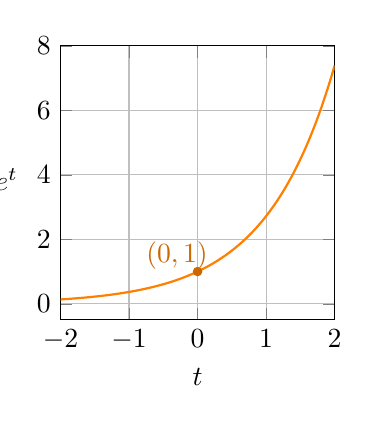
\begin{tikzpicture}
\begin{axis}[
    width=\dimexpr0.5\linewidth-1cm\relax,
    height=\dimexpr0.5\linewidth-1cm\relax,
    grid=both,
    unbounded coords=jump,
    title style={font=\small, yshift=0.6em},
    xlabel=$t$,
    ylabel style={%
        rotate=-90,
        anchor=east,
        overlay%
    },
    ylabel={$\varphi(t)=e^t$},
    xmin=-2, xmax=2,
    ymin=-0.5, ymax=8
]
\addplot[orange,thick,domain=-2:2,samples=200]{exp(x)};
\addplot[only marks, mark=*, mark size=1.5pt, orange!80!black] coordinates {(0,1)};
\node[orange!80!black] at (axis cs:-0.3,1.5) {$(0,1)$};
\end{axis}
\end{tikzpicture}
\end{center}
\end{enumerate}
\end{sol}



% Ejercicio 6
\begin{ejer}
Sean $f_1$ y $f_2$ dos funciones de clase $C^\infty$ en $\mathbb{R}^2$ y a valores en $\mathbb{R}$.
Supongamos que para todo $(t,x) \en \mathbb{R}^2$ se cumple que $f_1(t,x) \leq f_2(t,x)$.  
Demostrar que, si $\varphi_1 : I_1 \to \mathbb{R}$ es solución de la ecuación
$\dot{x} = f_1(t,x)$, $\varphi_2 : I_2 \to \mathbb{R}$ es solución de la ecuación
$\dot{x} = f_2(t,x)$, y además existe $t_0 \en I_1 \cap I_2$ tal que
$\varphi_1(t_0) = \varphi_2(t_0)$, entonces se cumple que
\[
    \varphi_1(t) \leq \varphi_2(t), \quad \forall \, t \en I_1 \cap I_2 \cap {]t_0, +\infty[}
\]
¿Qué ocurre si $t < t_0$?
\end{ejer}
\begin{sol}[Demostración]
Primero probemos la versión con las desigualdades estrictas (i.e.,  $f_1 < f_2$ implica $\varphi_1 < \varphi_2$), luego veremos que la versión que se pide se sigue por continuidad en las condiciones iniciales.
Denotemos $I \coloneqq I_1 \cap I_2$ y
\[
\varphi(t) \coloneqq \varphi_2(t) - \varphi_1(t), \quad t \in I
\]
Queremos probar que $\varphi(t) > 0$ para todo $t \in I \cap {]t_0,+\infty[}$, donde $\varphi(t_0)=0$.

Supongamos, por contradicción, que existe $t_1>t_0$ en $I$ con $\varphi(t_1)\leq0$. Luego, el conjunto
\[
A := \set*{ t>t_0 \given \varphi(t) \leq 0 }
\]
es no vacío, por lo que existe
\[
t^* := \inf A
\]
Como $\dot\varphi(t_0) = f_2(t_0, \varphi_1(t_0)) - f_1(t_0, \varphi_1(t_0)) > 0$ (pues $\varphi_1(t_0) = \varphi_2(t_0)$) se tiene que $t^* > t_0$ ya que $\varphi(t) > 0$ justo a la derecha de $t_0$; además, la continuidad de $\varphi$ asegura que 
\[
\varphi(t^*) = 0 \quad \text{y} \quad \varphi(t) > 0 \text{ para todo } t \in [t_0, t^*]
\]

Como $\varphi$ es diferenciable en $t^*$, la derivada izquierda (que es igual a la derivada) satisface
\[
\dot\varphi(t^{*-}) = \lim_{h \to 0^-} \frac{\varphi(t^*+h)-\varphi(t^*)}{h} \le 0
\]
ya que $\varphi(t^*+h) > 0$ con $h < 0$. Por otro lado, por definición de $\varphi$ y usando que $f_1 \le f_2$,
\[
\dot\varphi(t^*) = f_2(t^*, \varphi_2(t^*)) - f_1(t^*, \varphi_1(t^*)) = f_2(t^*, \varphi_2(t^*)) - f_1(t^*, \varphi_2(t^*)) > 0
\]
gracias a que $\varphi_1(t^*) = \varphi_2(t^*)$. Hemos llegado a una contradicción, por lo que no puede existir $t_1>t_0$ con $\varphi(t_1) \leq 0$, i.e.,
\[
\varphi_1(t) < \varphi_2(t), \quad t>t_0.
\]
\par
\emph{Ahora probemos la versión con desigualdades no estrictas:}\\
fijamos $t > t_0$ en $I_1 \cap I_2$. Para cada $\epsilon > 0$, definimos la función
\[
f_{2,\epsilon}(t,x) = f_2(t,x) + \epsilon.
\]
Dado que $f_2$ es de clase $C^\infty$, $f_{2,\epsilon}$ también es de clase $C^\infty$. Además, para todo $(t,x)$, se tiene
\[
f_1(t,x) \leq f_2(t,x) < f_2(t,x) + \epsilon = f_{2,\epsilon}(t,x),
\]
es decir, $f_1(t,x) < f_{2,\epsilon}(t,x)$. Sea $\varphi_{2,\epsilon}$ la solución de la ecuación diferencial $\dot{x} = f_{2,\epsilon}(t,x)$ con condición inicial $\varphi_{2,\epsilon}(t_0) = \varphi_2(t_0) = \varphi_1(t_0)$. Por el teorema de existencia y unicidad (dado que $f_{2,\epsilon}$ es suave), $\varphi_{2,\epsilon}$ está definida en un intervalo abierto que contiene a $t_0$. Para $\epsilon$ suficientemente pequeño, el intervalo de definición de $\varphi_{2,\epsilon}$ contiene al intervalo $I_1 \cap I_2 \cap [t_0, t]$ (por dependencia continua de las soluciones respecto a parámetros). Aplicando el resultado del Ejercicio 6 (con desigualdades estrictas) a $f_1$ y $f_{2,\epsilon}$, obtenemos que
\[
\varphi_1(s) < \varphi_{2,\epsilon}(s) \quad \text{para todo } s \en I_1 \cap I_2 \cap {]t_0, +\infty[}.
\]
En particular, para $s = t$, tenemos
\[
\varphi_1(t) < \varphi_{2,\epsilon}(t).
\]

Ahora, consideramos la familia de funciones $\{ f_{2,\epsilon} \}_{\epsilon > 0}$. Cuando $\epsilon \to 0$, $f_{2,\epsilon} \to f_2$ uniformemente en conjuntos compactos de $\mathbb{R}^2$. Por la dependencia continua de las soluciones respecto a parámetros, se tiene que $\varphi_{2,\epsilon} \to \varphi_2$ uniformemente en compactos del intervalo de definición de $\varphi_2$. En particular, para $t$ fijo,
\[
\lim_{\epsilon \to 0^+} \varphi_{2,\epsilon}(t) = \varphi_2(t).
\]
Dado que $\varphi_1(t) < \varphi_{2,\epsilon}(t)$ para todo $\epsilon > 0$, tomando el límite cuando $\epsilon \to 0$, obtenemos
\[
\varphi_1(t) \leq \varphi_2(t).
\]
Esto vale para todo $t > t_0$ en $I_1 \cap I_2$. Por continuidad, también vale para $t = t_0$ (donde $\varphi_1(t_0) = \varphi_2(t_0)$). Por lo tanto,
\[
\varphi_1(t) \leq \varphi_2(t) \quad \text{para todo } t \en I_1 \cap I_2 \cap [t_0, +\infty[.
\]

\emph{¿Qué pasa si $t < t_0$?}\\ 
Basta con considerar 
\[
    \psi_i(t) \coloneq \varphi_i(-t)%
    ,\quad%
    g_i(t,x) \coloneq -f_i(-t,x)%
    \quad\text{y}\quad%
    I'_i \coloneq \set{t \en \mathbb{R} \given -t \en I_i}%
    \quad\text{con}\quad%
    i = 1,2
\]
entonces $\psi_i(t)$ es solución de $\dot{x} = g_i(t,x)$ y se cumple que $g_2(t,x) \leq g_1(t,x)$ para cada $(t, x) \en \mathbb{R}^2$ donde además $\psi_2(-t_0) = \psi_1(-t_0)$. Por lo tanto, gracias a lo recién probado, $\psi_1(t) \geq \psi_2(t)$ para cada $t \en I' \cap {]{-t_0}, +\infty[}$, esto es, $\varphi_1(t) \geq \varphi_2(t)$ para cada $t \en I \cap {]{-\infty}, t_0[}$.

% Denotaremos $I \coloneq I_1 \cap I_2$ y $\varphi \coloneq \varphi_2 - \varphi_1$. Sea $t \en I \cap {]t_0, +\infty[}$ arbitrario, luego existe un intervalo $I_3$ abierto y acotado con $[t_0, t] \subseteq I_3 \subseteq \ubar{I_3} \subseteq I$ (pues $\mathbb{R}$ es localmente compacto) por lo que existen, gracias a la continuidad de $\varphi_1$ y $\varphi_2$,
% \[
%     a \coloneq \min_{t \en \scriptstyle{\overline{\vphantom{t}\smash{I_3}}}} \set{\varphi_1(t), \varphi_2(t)}%
%     \quad\text{y}\quad%
%     b \coloneq \max_{t \en \scriptstyle{\overline{\vphantom{t}\smash{I_3}}}} \set{\varphi_1(t), \varphi_2(t)}
% \]
% Como $f_2$ es de clase $C^{\infty}$, la parcial $\partial_xf_2$ es continua, así que existe
% \[
%     M \coloneq \min\set*{%
%         \partial_xf_2(s,x) \given (s,x) \en \ubar{I_3} \times [a,b]
%     }
% \]
% Ahora bien, notemos que por definición, para cada $s \en I_3$,
% \[
%     \dot\varphi(s) = f_2(s, \varphi_2(s)) - f_1(s, \varphi_1(s)) \geq f_2(s, \varphi_2(s)) - f_2(s, \varphi_1(s))
% \]
% pero por teorema del valor medio, existe un $\xi$ entre $\varphi_2(s)$ y $\varphi_1(s)$ tal que 
% \[
%     f_2(s, \varphi_2(s)) - f_2(s, \varphi_1(s)) = \partial_xf_2(s,\xi)\big(\varphi_2(s) - \varphi_1(s)\big) \geq M\varphi(s)
% \]
% por lo tanto, $\dot\varphi(s) \geq M\varphi(s)$ en $I_3$.\footnote{Notemos que para encontrar este $M$, basta con que $f_2$ sea localmente Lipschitz en $x$ de manera uniforme en $t$.} Consideremos ahora el factor $\mu(s) \coloneq e^{M(t_0 - s)}$ definido en $I_3$: esta función cumple que $\dot\mu = -M\mu$, por lo que, gracias a que $\mu > 0$, sobre $I_3$ se cumple
% \[
%     \dot{\varphi\mu}%
%     = \dot\varphi\mu + \varphi\dot\mu%
%     = \dot\varphi\mu - M\varphi\mu%
%     = (\dot\varphi - M\varphi)\mu%
%     \geq 0
% \]
% De esto se sigue que $\varphi\mu$ es monótona no decreciente, pero $\varphi(t_0)\mu(t_0) = 0$ y $t > t_0$, por lo tanto $\varphi(t)\mu(t) \geq 0$; más aún, como $\mu$ es siempre positiva, $\varphi(t) \geq 0$. Recordemos que $\varphi = \varphi_2 - \varphi_1$, entonces hemos probado que $\varphi_2(t) \geq \varphi_1(t)$ donde $t \en I \cap {]t_0, +\infty[}$ es arbitrario.\qedhere\par
¿Qué pasa si $t < t_0$? Basta con considerar 
\[
    \psi_i(t) \coloneq \varphi_i(-t)%
    ,\quad%
    g_i(t,x) \coloneq -f_i(-t,x)%
    \quad\text{y}\quad%
    I'_i \coloneq \set{t \en \mathbb{R} \given -t \en I_i}%
    \quad\text{con}\quad%
    i = 1,2
\]
entonces $\psi_i(t)$ es solución de $\dot{x} = g_i(t,x)$ y se cumple que $g_2(t,x) \leq g_1(t,x)$ para cada $(t, x) \en \mathbb{R}^2$ donde además $\psi_2(-t_0) = \psi_1(-t_0)$. Por lo tanto, gracias a lo recién probado, $\psi_1(t) \geq \psi_2(t)$ para cada $t \en I' \cap {]{-t_0}, +\infty[}$, esto es, $\varphi_1(t) \geq \varphi_2(t)$ para cada $t \en I \cap {]{-\infty}, t_0[}$.\par\vspace{1em}

\begin{nota}
    Para la prueba de las desigualdades estrictas, solo usamos que $f_1 < f_2$ en la imagen de alguna de las dos soluciones.
\end{nota}
\end{sol}


% Ejercicio 7
\begin{ejer}
Utilizando el ejercicio anterior, demostrar que toda solución maximal
de la ecuación
\[
    \dot{x} = t^2 + x^2
\]
está definida en un intervalo acotado.
\end{ejer}
\begin{sol}[Demostración]
Procedamos por contradicción suponiendo que existe una solución $\varphi$ definida sobre un intervalo $I$ no acotado. Existen dos posibilidades, que se extienda hasta $+\infty$ o hasta $-\infty$, veremos que ninguna es posible; pero antes, comparemos $\varphi$ con la solución maximal de $\dot{x} = t^2$: si $t_0 \en I$ es cualquier punto y $x_0 \coloneq \varphi(t_0)$, entonces la solución maximal de $\dot{x} = t^2$ que pasa por $(t_0, x_0)$ es
\[
    \psi(t) = x_0 + \frac13(t^3 - t_0^3), \quad \forall t \en \mathbb{R}
\]
por lo cual, como $t^2 + x^2 \geq t^2$, el \myref{ejer:1.6} garantiza que $\varphi(t) \geq \psi(t)$ con $t \en I \cap {]t_0, +\infty[}$ y que $\varphi(t) \leq \psi(t)$ con $t \en I \cap {]{-\infty}, t_0[}$.
    \begin{itemize}
    \item Si $I \supseteq {[a, +\infty[}$ para algún $a \en \mathbb{R}$, entonces $\varphi$ alcanza algún valor positivo, pues ya vimos que 
    \[
        \varphi(t) \geq \varphi(a) + \frac13(t^3 - a^3) \xrightarrow{t \to \infty} +\infty
    \]
    por lo cual existe $t_0 \geq a$ tal que $\varphi(t_0) > 0$, llámese $\varphi(t_0) = x_0$. Ahora comparemos con la EDO $\dot{x} = x^2$ para la condición inicial $(t_0,x_0)$ (como $x_0 > 0$ la unicidad garantiza que cualquier solución no trivial no toca el cero), 
    \[
        \frac{\dot{x}(t)}{x(t)^2} = 1%
        \implies \int^t_{t_0}\frac{\dot{x}(s)}{x(s)^2}\;\mathrm{d}s = t - t_0%
        \implies -\frac{1}{x(t)} + \frac{1}{x_0} = t - t_0
    \]
    por lo que $x(t) = \big(t_0 + x_0^{-1} - t\big)^{-1}$ es una solución de $\dot{x} = x^2$, la cual cumple $x(t_0) = x_0 = \varphi(t_0)$ y está definida sobre ${]a, T[}$ donde $T \coloneq t_0 + x_0^{-1} > t_0$; sin embargo, $t^2 + x^2 \geq x^2$, así que el \myref{ejer:1.6} implica que $\varphi(t) \geq x(t)$ en ${]t_0, T[}$; no obstante, 
    \[
        \varphi(t) \geq x(t) \xrightarrow{t\to T^-} +\infty
    \]
    Esto contradice que $\varphi$ esté definida y sea continua en $T \en [a, +\infty[$.

    \item Si $I \supseteq {]{-\infty}, a]}$ para algún $a \en \mathbb{R}$, entonces $\varphi$ alcanza un valor negativo, pues ya vimos que 
    \[
        \varphi(t) \leq \varphi(a) + \frac13(t^3 - a^3) \xrightarrow{t \to {-\infty}} {-\infty}
    \]
    por lo cual existe $t_0 \leq a$ tal que $\varphi(t_0) < 0$, llámese $\varphi(t_0) = x_0$. Ahora comparemos con la EDO $\dot{x} = x^2$ para la condición inicial $(t_0,x_0)$ (como $x_0 < 0$ la unicidad garantiza que cualquier solución no trivial no toca el cero), 
    \[
        \frac{\dot{x}(t)}{x(t)^2} = 1%
        \implies \int^t_{t_0}\frac{\dot{x}(s)}{x(s)^2}\;\mathrm{d}s = t - t_0%
        \implies -\frac{1}{x(t)} + \frac{1}{x_0} = t - t_0
    \]
    por lo que $x(t) = \big(t_0 + x_0^{-1} - t\big)^{-1}$ es una solución de $\dot{x} = x^2$ que cumple $x(t_0) = x_0 = \varphi(t_0)$ y está definida en ${]T, a[}$ donde $T \coloneq t_0 + x_0^{-1} < t_0$; sin embargo, $t^2 + x^2 \geq x^2$, así que el \myref{ejer:1.6} (el caso $t < t_0$) implica que $\varphi(t) \leq x(t)$ en ${]T, t_0[}$; no obstante, 
    \[
        \varphi(t) \leq x(t) \xrightarrow{t\to T^+} -\infty
    \]
    Esto contradice que $\varphi$ esté definida y sea continua en $T \en {]{-\infty}, a]}$.
    \end{itemize}
    En cualquier caso, el error estuvo en suponer que $I$ no es acotado.
\end{sol}



% Ejercicio 8
\begin{ejer}
Se considera la ecuación diferencial
\[
    \dot{x} = \cos(t+x).
\]
Probar que todas las soluciones maximales están definidas en $\mathbb{R}$.  
Hallar los máximos, mínimos y puntos de inflexión de las mismas.
\end{ejer}
\begin{sol}[Demostración]
% Procedamos por contradicción suponiendo que $\varphi$ es solución maximal sobre $I \neq \mathbb{R}$ que pasa por $(t_0, x_0)$. Como $\dot{\varphi} \leq 1$, $\varphi$ es Lipschitz con constante 1, así que es uniformemente continua; luego, para cualquier ${]a, b[} \subseteq I$ con $t_0 \en {]a, b[}$, se tiene que $\varphi({]a, b[})$ es acotado; sin embargo, el teorema de escape de compactos implica que existen $t_1 < t_0 < t_2$ en $I$ tales que 
% \[
%     (t_1, \varphi(t_1)), (t_2, \varphi(t_2)) \notin [a,b] \times \ubar{\varphi({]a, b[})}
% \]
% como $\varphi(t_1), \varphi(t_2) \en \ubar{\varphi({]a, b[})}$, forzosamente $t_1, t_2 \notin [a,b]$, i.e., $t_1 <a$ y $t_2 >b$. Ya sea que exista $b' \coloneq \sup I$ o $a' \coloneq \inf I$, hemos llegado a una contradicción, pues en cualquier caso existen $t_1, t_2 \en I$ con $t_1 <a$ y $t_2 > b$.

Procedamos por contradicción, suponiendo que hay una solución maximal $\varphi$ definida en $I \coloneq {]a,b[}$ donde $b \en \mathbb{R}$ y $a \en {[{-\infty}, b[}$ (el caso $a \en \mathbb{R}$ y $b \en {]a, +\infty]}$ es análogo). Como $\dot{\varphi} \leq 1$, $\varphi$ es Lipschitz con constante 1 así que es uniformemente continua; luego, es un teorema bien conocido que $\varphi$ se puede extender de forma continua a una función $\ubar{\varphi}$ definida sobre $]a,b]$. Sin embargo, el teorema de existencia y unicidad garantiza que existe una solución de la EDO $\psi$ definida en un entorno $J$ de $b$ que pasa por $(b, \ubar{\varphi}(b))$, como $\dot{\varphi}$ es continua se tiene que
\[
    \dot{\ubar{\varphi}}(b^-) = \lim_{t \to b^-} \dot\varphi(t) = \cos(b + \ubar{\varphi}(b))
\]
por lo que la siguiente función es solución de la EDO en $I \cup J \supset I$
\[
    \phi(t) =%
    \begin{cases}
        \ubar{\varphi}(t), &\text{si } t \en {]a,b]}\\
        \psi(t), &\text{si } t \en J \setminus {]a,b]}
    \end{cases}
\]
Esto contradice la maximalidad de $\varphi$, el error estuvo en suponer que hay una solución maximal no definida en todo $\mathbb{R}$.

\vspace{1em}
\emph{Ahora encontremos lo máximos, mínimos y puntos de inflexión de las soluciones:}\\
Los máximos y mínimos se producen cuando $\dot{\varphi}(t) = \cos(t+\varphi(t)) = 0$, es decir,
\[
    t + \varphi(t) = \frac{\pi}{2} + k\pi, \quad k \en \mathbb{Z}
\]
Para distinguir máximo o mínimo, consideramos la segunda derivada:
\[
    \ddot{\varphi}(t) = -\sin(t+\varphi(t)) \cdot (1 + \dot{\varphi}(t)) = -\sin(t+\varphi(t)) \cdot \big(1 + \cos(t+\varphi(t))\big)
\]
En los puntos críticos, $\cos(t+\varphi(t))=0$, así que
\[
    \ddot{\varphi}(t) = -\sin(t+\varphi(t)) = -\sin(\nicefrac{\pi}{2} + k\pi) = (-1)^{k+1}
\]
por lo tanto:
\begin{itemize}
    \item Si $k$ es par, $\ddot{\varphi}(t)<0$ y $t$ es máximo local.
    \item Si $k$ es impar, $\ddot{\varphi}(t)>0$ y $t$ es mínimo local.
\end{itemize}
Los puntos de inflexión se producen cuando $\ddot{\varphi}(t)=0$, es decir, cuando
\[
    \sin(t+\varphi(t)) = 0 \quad \text{o} \quad \cos(t+\varphi(t))=-1
\]
lo que equivale a
\[
    t + \varphi(t) = k\pi \quad \text{o} \quad t + \varphi(t) = \pi + 2k\pi, \quad k \en \mathbb{Z}
\]

En conclusión, la solución oscila siguiendo líneas de la forma $t + \varphi(t) = \text{constante}$, alternando máximos y mínimos cada $\pi$, y presentando puntos de inflexión donde cambia la concavidad.
\end{sol}



% Ejercicio 9
\begin{ejer}
Estudiaremos ahora cualitativamente la ecuación diferencial
\[
    \dot{x} = t - x^2.
\]
\begin{enumerate}[label = (\alph*)]
    \item Hallar los máximos, mínimos y puntos de inflexión de las soluciones.
    
    \item Demostrar que para toda solución $\varphi = \varphi(t)$ existe un instante
    $T \geq 0$ (que depende de $\varphi$) tal que $\varphi(t) < \sqrt{t}$ para todo $t > T.$
    
    \item Llamamos ahora $\varphi_c$, para cada $c \en \mathbb{R}$, a la solución maximal que
    verifica $\varphi_c(0) = c$. Probar las siguientes afirmaciones:
    \begin{itemize}
        \item Si $c \geq 0$ entonces $\varphi_c$ está definida para todo $t > 0$.
        \item Existe $k < 0$ tal que para todo $c < k$ la solución $\varphi_c$ tiende a $-\infty$ en tiempo finito.
        \item Existe un único valor $c_0$ tal que $\varphi_{c_0}$ está definida para todo $t > 0$ y
        \[
            \lim_{t \to \infty} \big( \varphi_{c_0}(t) + \sqrt{t} \big) = 0.
        \]
    \end{itemize}
\end{enumerate}
\end{ejer}
\begin{sol}
    \begin{enumerate}[label = (\alph*)]
    \item Sea $\varphi$ una solución cualquiera de $\dot x = t - x^2$, entonces:
    \[
        \dot\varphi(t)=t-\varphi(t)^2%
        \quad\text{y}\quad%
        \ddot\varphi(t) = 1-2\varphi(t)\dot\varphi(t) = 1-2\varphi(t)(t-\varphi(t)^2)
    \]
    \emph{Puntos críticos:}
    los puntos críticos ocurren cuando $\dot\varphi(t)=0$, es decir
    \[
    t-\varphi(t)^2=0 \quad\Longleftrightarrow\quad \varphi(t)=\pm\sqrt{t}
    \]
    lo cual sólo tiene sentido para $t\ge 0$. Por tanto, los instantes críticos corresponden a las intersecciones de la solución con la parábola $x=\pm\sqrt{t}$. Más aún, si $t_0$ es punto crítico,
    \[
    \ddot\varphi(t_0)=1-2\varphi(t_0)\cdot 0 = 1
    \]
    por lo que $\ddot\varphi(t_0) > 0$ y $t_0$ es un mínimo local, i.e., no hay máximos locales.\par
    \emph{Puntos de inflexión:}
    los puntos de inflexión ocurren cuando $\ddot\varphi(t)=0$; es decir, cuando
    \[
    1-2\varphi(t)(t-\varphi(t)^2) = 0
    \quad\iff\quad
    2\varphi(t)\bigl(t-\varphi(t)^2\bigr)=1
    \]
    es decir, para un punto de inflexión $(t,\varphi(t))$ debe cumplirse
    \[
    t = \varphi(t)^2 + \frac{1}{2\varphi(t)}, \qquad \varphi(t)\neq 0
    \]
    Por tanto, los puntos de inflexión se encuentran en la siguiente curva de $\mathbb{R}^2$ 
    \[
    \mathcal{C}= \set*{(t,x)\en\mathbb{R}^2 \given x\neq 0,\; t = x^2 + \tfrac{1}{2x}}
    \]
    
    \item \emph{Nota:} recordemos que en la prueba del \myref{ejer:1.6} solo usamos que $f_1 < f_2$ en la imagen de alguna de las soluciones.
    
    Sea $\varphi$ una solución definida en un intervalo $I$; más aún, podemos suponer sin perder generalidad que $I$ se extiende hasta $+\infty$, pues de no ser así, la proposición se cumple por vacuidad tomando $T \coloneq \max I$. Veamos primero que no es posible que $\varphi(t) > \sqrt{t}$ para cada $t \en I \cap \mathbb{R}^+$: en efecto, pues esto implicaría que $\varphi(t)^2 > \sqrt{t}^2 = t$ y por tanto
    \[
        \dot{\varphi}(t) = t - \varphi(t)^2 < 0
    \]
    pero esto implicaría que $\varphi$ es decreciente y al mismo tiempo $\varphi(t) > \sqrt{t} \xrightarrow{t \to \infty} +\infty$, lo cual es absurdo. Hemos probado que tiene que existir un $t_0 \en I \cap \mathbb{R}^+$ tal que $\varphi(t_0) \leq \sqrt{t_0}$. Ahora bien, gracias la continuidad de $\varphi$, o bien se cumple que $\varphi(t) < \sqrt{t}$ para cada $t \en I \cap \mathbb{R}^+$ (en cuyo caso ya terminamos), o bien existe $t_1 \en I \cap \mathbb{R}^+$ tal que $\varphi(t_1) = \sqrt{t_1}$ (pues si tuviéramos algún $t$ con $\varphi(t) > \sqrt{t}$, el teorema del valor intermedio garantizaría que existe el $t_1$ que buscamos). Por este motivo , podemos suponer que se cumple $\varphi(t_1) = \sqrt{t_1}$ para algún $t_1 \en I \cap \mathbb{R}^2$; sin embargo, la función $\sqrt{t}$ es solución de $\dot{x} = (2x)^{-1}$ y además
    \[
        t^2 - (\sqrt{t})^2 = 0 < (2\sqrt{t})^{-1}
    \]
    por lo cual, el \myref{ejer:1.6} (recordemos la nota del inicio) implica que $\varphi(t) < \sqrt{t}$ con $t > t_0$. 
    
    \item 
    \begin{itemize}
        \item Supongamos por contradicción que $I_c$ es el dominio de $\varphi_c$ y $b \coloneq \sup I_c < +\infty$, entonces, como consecuencia directa del teorema de escape de compactos,
        \[
        \lim_{t \to b^-} |\varphi_c(t)| = +\infty
        \]
        Veamos ahora que esto es imposible porque existen cotas uniformes que impiden tanto el crecimiento hacia $+\infty$ como la ca\'ida hacia $-\infty$.
    
        Primero, para la cota superior observamos que
        \[\varphi_c'(t)=t-\varphi_c(t)^2\le t\qquad(\forall t \en I_c)\]
        de modo que integrando entre $0$ y $t$ se obtiene
        \[\varphi_c(t)\le c+\int_0^t s\,ds=c+\tfrac{t^2}{2}\]
        En particular $\varphi_c(t)$ no puede divergir a $+\infty$ en tiempo finito.
        
        Para la cota inferior notemos que su $c > 0$, entonces $\varphi_c$ se mantiene mayor o igual a cero, pues en otro caso tendría (por continuidad) que existir $t_1 > 0$ tal que $\varphi_c(t_1) = 0$, por lo que $\dot{\varphi_c}(t_1) = t_1 > 0$ así que jamás puede tocar al eje cero "bajando". De forma similar, el caso $c = 0$ la función se mantiene justo a la derecha dentro de la zona donde la derivada es positiva (el lado derecho de la parábola $\pm\sqrt{t}$) por lo que la función alcanza un valor positivo justo a la derecha y repetir el argumento anterior para probar que la función no se hace negativa. En cualquier caso, no puede explotar a $-\infty$.

        \item El argumento consiste en comparar localmente la ecuaci\'on con la EDO explotante $y'=-\tfrac12 y^2$. Fijemos $\varepsilon>0$ (por ejemplo $\varepsilon=1$) y consideremos el intervalo $[0,\varepsilon]$. Si $x\le-\sqrt{2\varepsilon}$ y $t\in[0,\varepsilon]$ entonces
        \[t-x^2\le\varepsilon-x^2\le-\tfrac12 x^2\]
        Tomemos $k:=-\sqrt{2\varepsilon}<0$ y consideremos $c<k$. Por continuidad de la soluci\'on existe un intervalo inicial en el que $\varphi_c(t)\le-\sqrt{2\varepsilon}$ (pues $\varphi_c(0)=c$ ya es m\'as negativo que $-\sqrt{2\varepsilon}$). Mientras $\varphi_c(t)\le-\sqrt{2\varepsilon}$ y $t\in[0,\varepsilon]$ se cumple
        \[\varphi_c'(t)=t-\varphi_c(t)^2\le -\tfrac12\varphi_c(t)^2\]
        Sea ahora $y(t)$ la soluci\'on de
        \[y'=-\tfrac12 y^2,\qquad y(0)=c\]
        La soluci\'on expl\'icita es
        \[y(t)=\frac{2c}{ct+2}=\frac{c}{1+(c/2)t}\]
        y para $c<0$ tiene singularidad en tiempo finito $T=-2/c>0$ (es decir $y(t)\to-\infty$ cuando $t\to T^-$). Por el teorema de comparaci\'on, mientras ambas soluciones existan y se mantenga la condici\'on $\varphi_c(t)\le-\sqrt{2\varepsilon}$ se tiene $\varphi_c(t)\le y(t)$. Dado que $y$ explota a $-\infty$ en tiempo finito, la funci\'on $\varphi_c$ tambi\'en debe explotar (al menos tan pronto como $y$). Por tanto existe un valor $k<0$ (por ejemplo $k=-\sqrt{2}$ si elegimos $\varepsilon=1$) tal que para todo $c<k$ la soluci\'on maximal $\varphi_c$ tiende a $-\infty$ en tiempo finito. 

        \item Definimos
        \[G:=\{c\in\mathbb R:\ \varphi_c\text{ est\'a definida para todo }t>0\}\]
        (es decir, el conjunto de condiciones iniciales que producen soluciones globales hacia la derecha). Por el primer sub-inciso sabemos que $[0,\infty)\subset G$, luego $G\neq\emptyset$. Por el segundo sub-inciso, existe $k<0$ tal que $(-\infty,k)\cap G=\emptyset$, luego $G$ est\'a acotado inferiormente; en particular el infimo
        \[c_0:=\inf G\in\mathbb R\]
        est\'a bien definido y finito.
        
        Sea $(c_n)$ una sucesi\'on decreciente de elementos de $G$ con $c_n\to c_0$. Fijemos $T>0$. Para cada $n$ la soluci\'on $\varphi_{c_n}$ est\'a definida en $[0,T]$. Queremos mostrar que la familia $\{\varphi_{c_n}\}_n$ est\'a uniformemente acotada en $[0,T]$, lo que permitir\'a pasar a un l\'imite y usar la dependencia continua con respecto a la condici\'on inicial para obtener una soluci\'on definida en $[0,T]$ con valor inicial $c_0$; como $T>0$ es arbitrario, esto dar\'a la globalidad de $\varphi_{c_0}$.
        
        Primero, por la desigualdad ya vista, para todo $n$ y todo $t\in[0,T]$ se tiene
        \[\varphi_{c_n}(t)\le c_n+\tfrac{t^2}{2}\le c_1+\tfrac{T^2}{2},\]
        esto da una cota superior uniforme. Supongamos ahora que no existiera una cota inferior uniforme en $[0,T]$: entonces existir\'ia $t_0\in[0,T]$ y una subserie (todav\'ia denotada $c_n$) tal que $\varphi_{c_n}(t_0)\to-\infty$ cuando $n\to\infty$. Sea $M>0$ grande y elijamos $n$ tal que $\varphi_{c_n}(t_0)\le -M$. Aplicando el argumento del segundo sub-inciso (comparando con la ecuaci\'on $y'=-\tfrac12y^2$) se ve que si $M$ es suficientemente grande la soluci\'on que toma el valor $-M$ en $t_0$ explotar\'a a los pocos instantes (en un tiempo menor que $T-t_0$), lo que contradice que $\varphi_{c_n}$ est\'a definida en todo $[0,T]$. Por tanto la familia $\{\varphi_{c_n}\}_n$ est\'a acotada uniformemente en $[0,T]$.
        
        De esta acotaci\'on uniforme y de la dependenci\'on continua de la soluci\'on respecto de la condici\'on inicial (teorema de continuidad respecto a datos iniciales en problemas de valor inicial), se deduce que la sucesi\'on $\varphi_{c_n}$ converge uniformemente en $[0,T]$ hacia una soluci\'on $\varphi$ de la EDO con $\varphi(0)=c_0$. Como $T>0$ era arbitrario, esta soluci\'on est\'a definida en todo $[0,\infty)$ y por maximalidad de las $\varphi_c$ coincide con $\varphi_{c_0}$. Por tanto $c_0\in G$ y $\varphi_{c_0}$ es global.
        
        Sea $\varphi:=\varphi_{c_0}$. Introduzcamos el error respecto de la rama $-\sqrt t$:
        \[\varepsilon(t):=\varphi(t)+\sqrt t.\]
        Una cuenta directa sustituyendo $\varphi=-\sqrt t+\varepsilon$ en la ecuaci\'on da
        \begin{align*}
        \dot\varphi &= t-\varphi^2 \\ 
        -\tfrac{1}{2\sqrt t}+\dot\varepsilon &= t-\big(t-2\varepsilon\sqrt t+\varepsilon^2\big)=2\varepsilon\sqrt t-\varepsilon^2, \\
        \end{align*}
        luego
        \begin{equation}\label{eq:eps}
        \dot\varepsilon(t)=2\sqrt t\,\varepsilon(t)-\varepsilon(t)^2+\frac{1}{2\sqrt t}.
        \end{equation}
        
        Supondremos que $\varepsilon(t)$ no tiende a $0$ cuando $t\to\infty$ y obtendremos contradicci\'on. Si existiera una subsucesi\'on con l\'imite $L>0$, entonces para $t$ grande la ecuaci\'on aproximada
        \[\dot\varepsilon\approx 2\sqrt t\,\varepsilon
        \]
        indica que $\varepsilon$ crecer\'ia exponencialmente (con tasa proporcional a $\int^t\!\sqrt s\,ds\sim \tfrac23 t^{3/2}$), lo cual es incompatible con que $\varphi$ siga siendo una soluci\'on global de la EDO (en particular le llevar\'ia a cruzar hacia valores positivos y escapar de la vecindad de $-\sqrt t$). Si en cambio existiera una subsucesi\'on con l\'imite $L<0$, entonces para $t$ grande $\varepsilon$ ser\'ia suficientemente negativa y la desigualdad aproximada mostr\'aria que $\dot\varepsilon$ es muy negativa, llevando a explosiones hacia $-\infty$ en tiempo finito; esto contradice la globalidad de $\varphi$. Por estos dos motivos el \'unico valor posible para un l\'imite (si existe) es $0$.
        
        Para formalizar la existencia del l\'imite y que sea $0$ se puede proceder con una versi\'on refinada del argumento de shooting: si $c>c_0$ entonces $\psi:=\varphi_c-\varphi_{c_0}$ es positiva y satisface (al menos para $t$ grandes) una ecuaci\'on linealizada del tipo
        \[\dot\psi\approx 2\sqrt t\,\psi,\]
        que crece r\'apidamentey empuja a $\varphi_c$ lejos de la rama negativa; en particular para $c>c_0$ se tiene $\limsup_{t\to\infty}(\varphi_c(t)+\sqrt t)>0$. Por otra parte, para $c<c_0$ la soluci\'on explota en tiempo finito. Por continuidad estricta de la dependencia de la soluci\'on respecto de la condici\'on inicial (y por monotonicidad en la condici\'on inicial), existe entonces un valor cr\'itico $c_0$ tal que precisamente para $c=c_0$ la soluci\'on queda aislada y verifica
        \[\lim_{t\to\infty}\big(\varphi_{c_0}(t)+\sqrt t\big)=0.\]
        La unicidad de tal $c_0$ se sigue de la monotonicidad: si hubiera $c_1>c_0$ con la misma propiedad, entonces por monotonicidad $\varphi_{c_1}(t)>\varphi_{c_0}(t)$ para todo $t$, lo que impedir\'ia que ambas tuvieran la misma correcci\'on $o(1)$ respecto de $-\sqrt t$ cuando $t\to\infty$.\qedhere
    \end{itemize}
    \end{enumerate}
\end{sol}
